
Simulation settings
\begin{itemize}
  \item		job: mean duration:10sec, mean 3 containers,
        mean frontend 30 Mbps, mean backend 60 Mbps
  \item		node: capacity 30 containers
  \item		link: capacity 1000Mbps
  \item		user: mean job request: 1/20 job/sec
  \item		data: 1 data object/job (for simplicity)
  \item		simulate: 100 users for 1000 sec on topology in Figure \ref{fig:topology-simple}.
  \item		users and data objects are randomly assigned to nodes.
\end{itemize}

\begin{figure}[htb]
  \begin{center}
    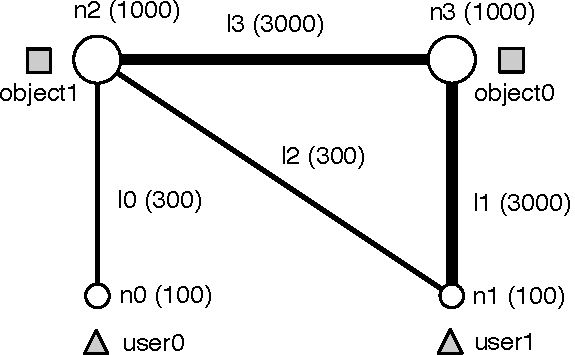
\includegraphics[width=7.5cm,clip]{topology-simple.pdf}
    \vspace{-2.0ex}
    \caption{simple simulation topology}
    \label{fig:topology-simple}
  \end{center}
\end{figure}

Simulation scenarios:

\begin{enumerate}
  \item	{\bf node only:} 4 nodes without randomization to show how the
        cost function works
  \item	{\bf link only:} 4 links without randomization to show
        different costs affects
  \item	{\bf monotonic function:} same as above but use monotonic cost
        function.
  \item	{\bf randomize:} 4 nodes and 4 links with randomization
  \item	{\bf surge:} same as above but with a request surge at one location
  \item	{\bf complex?:} realistic scenario
\end{enumerate}
